%!TEX root = main.tex

\section{Results and findings}
\label{sec:results-findings}

In this section, we present an analysis of the interplay between botness, political behavior (polarization and engagement) and influence.
In Sec.~\ref{subsec:polarization-botness}, we first profile the activity of users in the four reference populations; next, we analyze the political polarization and engagement, and their relation with the botness measure.
Finally, in Sec.~\ref{subsec:user-influence-results} we tabulate user influence against polarization and botness, and we construct \emph{the polarization map}.

%!TEX root = main.tex

\begin{figure}[!tb]
	\centering
	{
	\newcommand\myheight{0.145}
	\subfloat[] {
		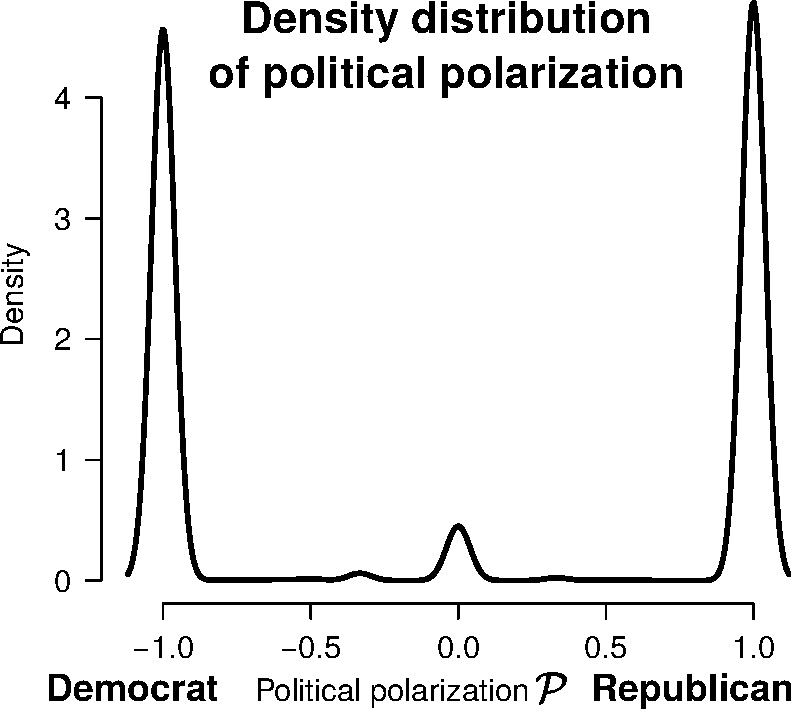
\includegraphics[height=\myheight\textheight]{a-density-distribution-political-bias}
		\label{subfig:distribution-political-bias}
	}
	\subfloat[] {
		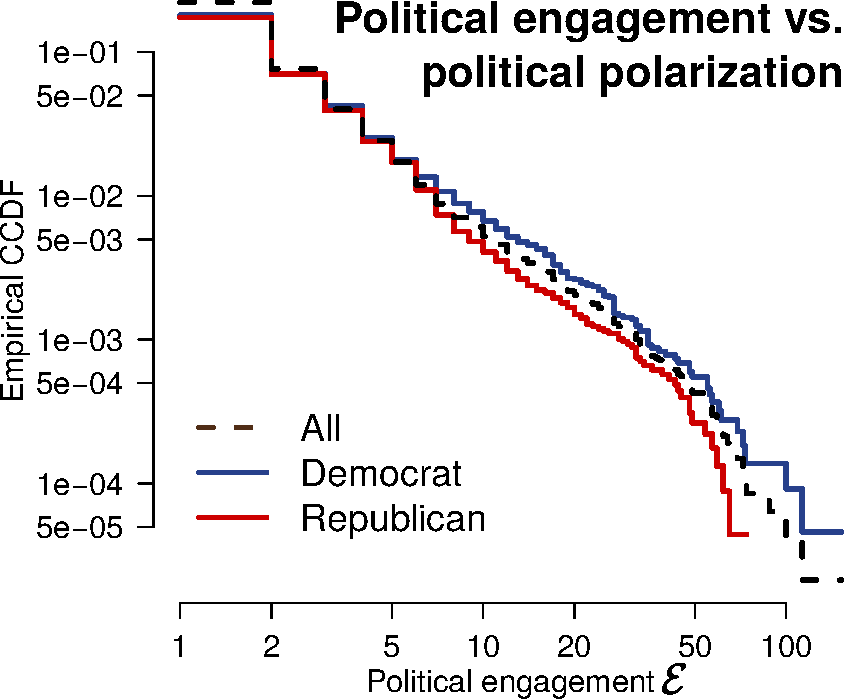
\includegraphics[height=\myheight\textheight]{b-CCDF-bias_engagement-vs-political-bias}
		\label{subfig:engagement-vs-political}
	}}
	\\
	{
	\newcommand\myheight{0.16}
	\subfloat[] {
		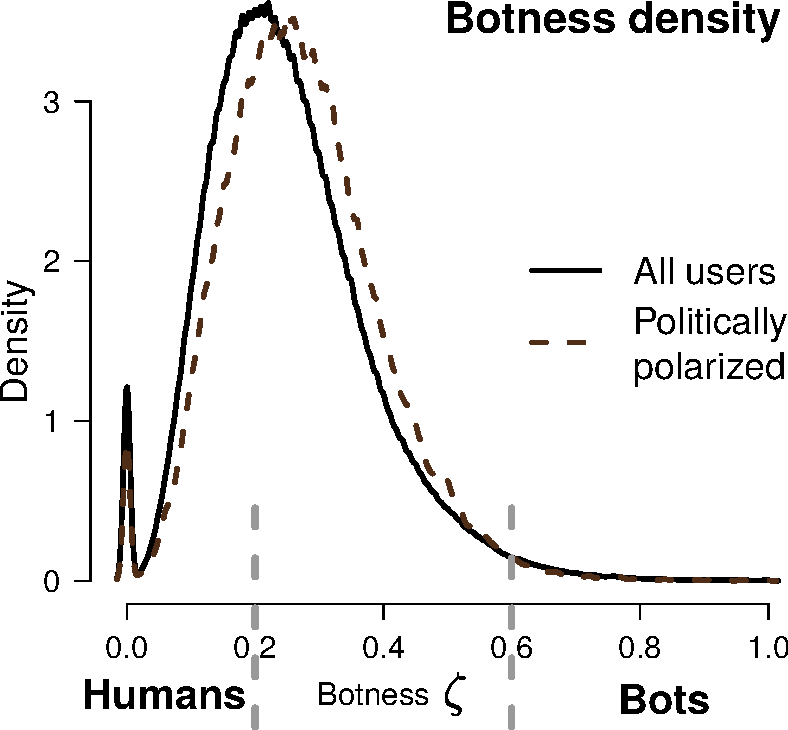
\includegraphics[height=\myheight\textheight]{botscore-density-all-polarization}
		\label{subfig:botscore-density}
	}
	\subfloat[] {
		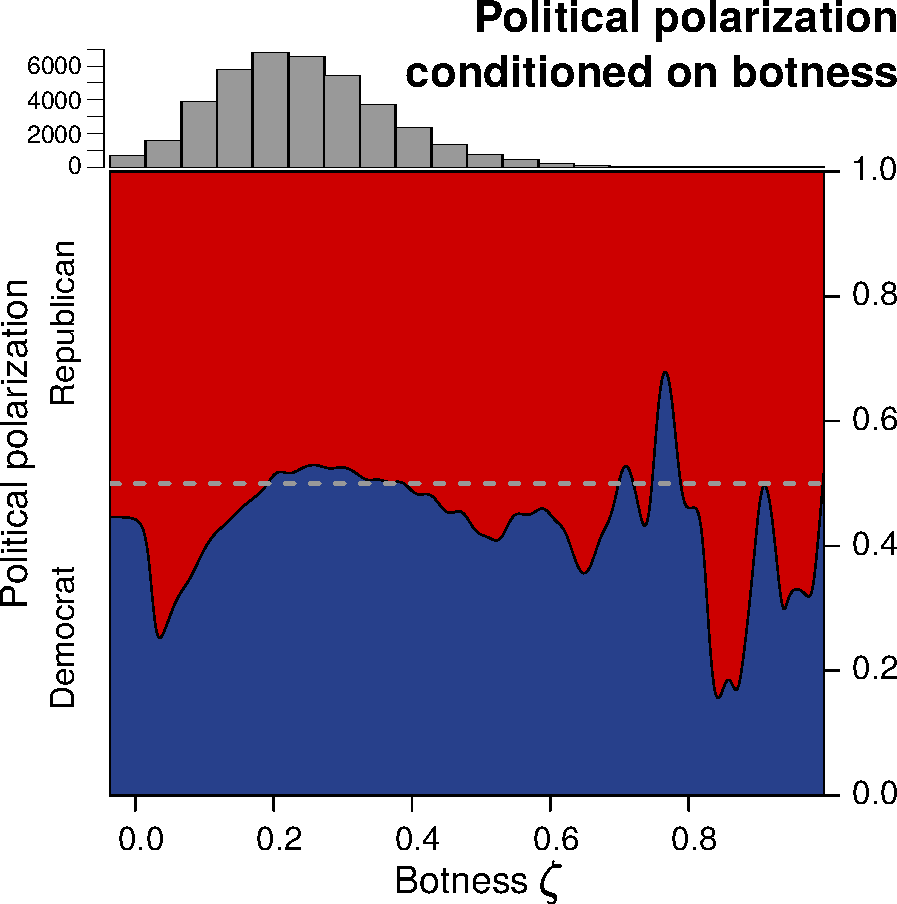
\includegraphics[height=\myheight\textheight]{botscore-conditional-density}
		\label{subfig:botscore-conditional-density}
	}}
	\\
	{ 
	\newcommand\myheight{0.145}
	\subfloat[] {
		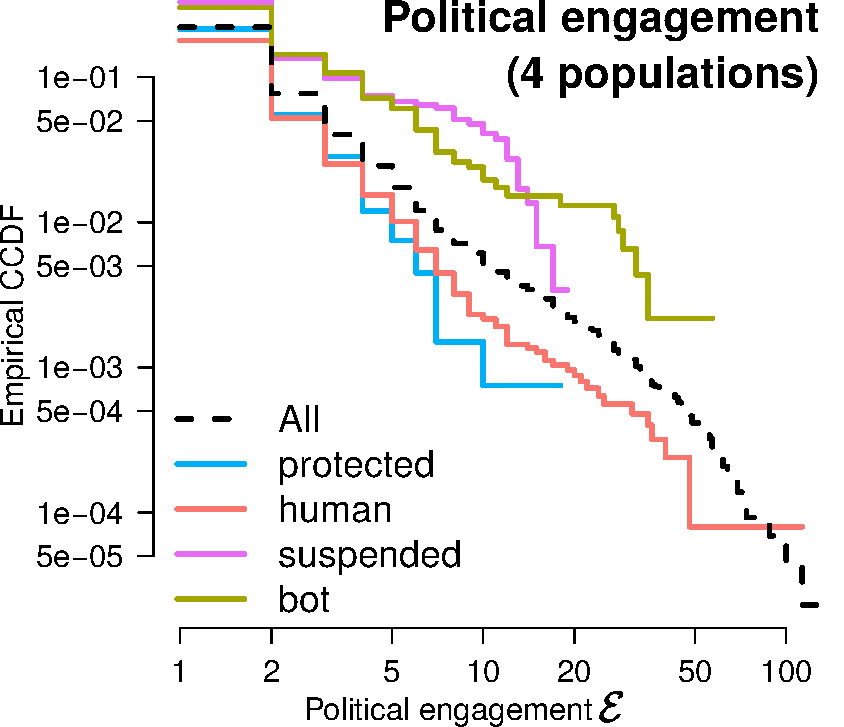
\includegraphics[height=\myheight\textheight]{c-pol-engagement-vs-botscore}
		\label{subfig:engagement-vs-botscore}
	}
	\subfloat[] {
		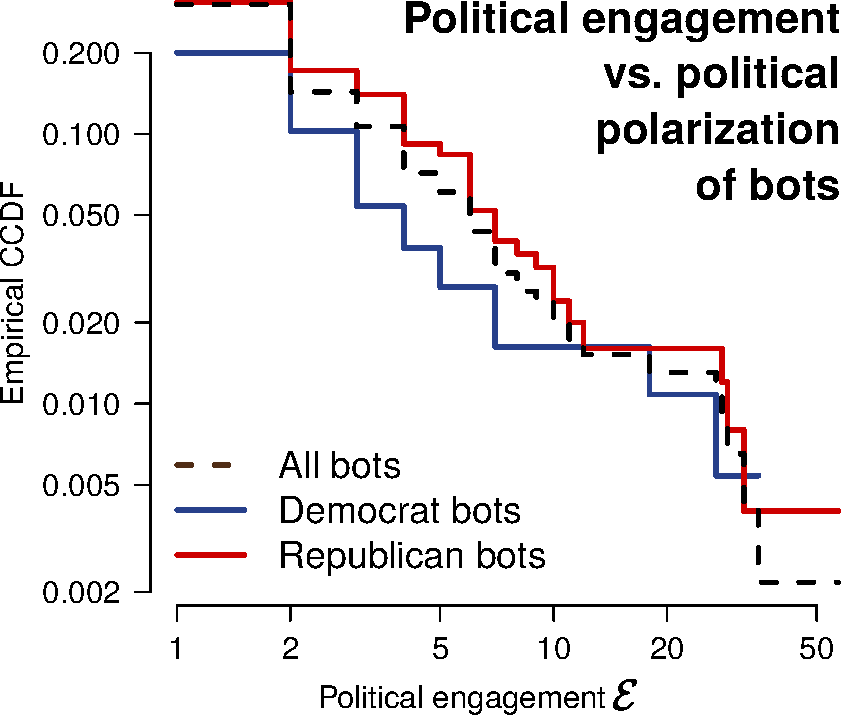
\includegraphics[height=\myheight\textheight]{d-BOTS_pol-engagement-vs-botscore}
		\label{subfig:BOTS_pol-engagement-vs-botscore}
	}
	}
	\caption{ 
		Political polarization, engagement and botness.
		\textbf{(a)} The density distribution of political polarization $\mathcal{P}$. %shows two peaks at -1 and 1, corresponding to strongly democrat and strongly republican respectively.
		\textbf{(b)} Log-log plot of the CCDF of political engagement $\mathcal{E}$ 
%		overall (dashed line), and 
		for the Democrat and Republican populations.
		% (blue and red lines respectively).
		%complementary cumulative distribution function shows that the political engagement score is long-tail distributed, with democrats being slightly more engaged than republicans overall.
		\textbf{(c)} The density distribution of botness $\zeta$ for the entire population (solid line) and the politically polarized population (dashed line). 
		%shows a large peak around $[0.1, 0.4]$ and a long tail.
		%Politically polarized users have slightly higher bot scores.
%		The dashed gray vertical lines show the threshholds for constructing the references human population ($\zeta \in [0, 0.2]$) and bot population ($\zeta \in [0.6, 1]$).
		\textbf{(d)} The conditional density of polarization conditioned on botness.
		The top panel shows the volumes of politically polarized users in 30 bins.
		\textbf{(e)(f)} CCDF of political engagement for the reference populations (e) and for the polarized \Bot populations (f).
		%\TODO{MAR}{Message in text: the \mbox{\Bot} and \mbox{\Suspended} populations are more politically engaged than the \mbox{\Human} and \mbox{\Protected}.}
	}
	\label{fig:bot-polarization}
%	\captionmoveup
\end{figure}

\subsection{Political behavior of humans and bots}
\label{subsec:polarization-botness}

\textbf{Twitter activity across four populations.}
We measure the behavior of users in the four reference populations defined in Sec.~\ref{subsec:political-polarization-measures} using several measures computed from the Twiter API.
The number of cascades started (i.e., number of original tweets) and the number of posted retweets are simple measures of activity on Twitter, and they are known to be long-tail distributed~\cite{Cha2010}.
%\TODO{RJA}{Am I correct that number of cascades initiated is the same thing as the number of original tweets authored during the 2 hours, since we saw previously that a cascade can have length of zero? Also I'm clarifying in previous sentence that "number of retweets" is the retweets sent/made, not received?. Finally, not a big deal but do we really expect that number of cascades initiated in 2 hour period would be power law distributed?  I expect it would be unequally distributed, but not long-tail.  Not big deal...}
Fig.~\ref{subfig:no-cascades} and~\ref{subfig:no-retweets} respectively plot the log-log plot of the empirical Complementary Cumulative Distribution Function (CCDF) for each of the two measures.
It is apparent that users in the \Bot and \Suspended populations exhibit higher levels of activity than the general population, whereas the \Human and \Protected populations exhibit lower level.
Fig.~\ref{subfig:numfolowers-CCDF} and~\ref{subfig:numfolowers-boxplot} plot the number of followers and present a more nuanced story:
the average bot user has 10 times more followers than the average human user;
however, bots have a median of $190$ followers, less than the median $253$ followers of human users.
In other words, some bots are very highly followed, but most are simply ignored.
Finally, Fig.~\ref{subfig:numfavorited} shows that bots favorite less than humans, indicating that their activity patterns differ from those of humans.
%\TODO{RJA}{I would get rid of Figure 6e since not really important to the story, and we are struggling to get it under 10 pages, not that it will save much.}
%
%the bot score against user political polarization (see Sec.~\ref{subsec:political-polarization-measures} and~\ref{subsec:political-polarization-results}) --, and against a number of measures provided by the Twitter API -- the number of followers, the number of friends, the number of favorited, the number of cascades initiated and the number of retweets. 
%
%\TODO{MAR}{Warning: outdated story. Check \mbox{Fig.~\ref{fig:bot-profiling}} for updated story.}
%\verify{
%Story here goes like this:
%\begin{itemize}
%	\item bots tend to be more active on Twitter, they start more cascades and they retweet more (Fig~\ref{subfig:tweets-vs-botscore} and~\ref{subfig:retweets-vs-botscore} respectively); 
%	mean number of cascades per bot is 2, and 2.3 for the suspended versus 1.1 for humans and 1.1 for protected;
%	the distribution of number of started cascades and retweets has a longer tail for bots than the general population and for humans.
%
%%	\item it is known that the distribution of number of followers and friends (users followed by a given users) is long tail.
%	However, the distributions for the bot and suspended populations are even more skewed: the median number of followers for a bot is $190$ (less than the average user of ), but the mean is $20,572$ (ten times more than the average user).
%	This indicates that most bots are not followed, while few get considerable following;
%	
%%	\item bots tend to favorite less than the average users (Fig.~\ref{subfig:numfavorited-vs-botscore}).
%\end{itemize}
% }
%
%This section profiles three of the measures proposed in Sec.~\ref{sec:four-measures}: the botness, the political polarization and the political engagement.
%the bot score against user political polarization (see Sec.~\ref{subsec:political-polarization-measures} and~\ref{subsec:political-polarization-results}) --, and against a number of measures provided by the Twitter API -- the number of followers, the number of friends, the number of favorited, the number of cascades initiated and the number of retweets. 
%A number of finding emerge from the analysis in presented in Fig.~\ref{fig:bot-polarization}, particularly about the polarization and engagements of bot-like accounts.

%\verify{RJA comment: Some fairly minor comments on Figure 5...In 5a there should be $\mathcal{P}$ after "Political polarization" on the x-axis. I think a better title for 5f is "Political engagement vs political polarization of bots" or similar.}

%\verify{RJA comment: Minor comment on Figure 7 - I don't think the labeling of the color scale is correct? If the colour shows the ratio of the densities of pop of D and R, shouldn't it range from 0 to infinity or something, but not +1 to -1.}

\textbf{Political polarization and engagement.}
The density distribution of political polarization (Fig.~\ref{subfig:distribution-political-bias}) shows two peaks at -1 and 1, corresponding to strongly pro-Democrat and strongly pro-Republican respectively. 
The shape of the density plot is consistent with the sizes of Republican and Democrat populations (Sec.~\ref{subsec:political-polarization-measures}), and the extreme bi-modality can be explained by the clear partisan nature of the chosen hashtags and by the known political polarization of users on Twitter \cite{conover.2011,barbera.2015}, which will be greatly enhanced in the context of a political debate.
%This validates our political polarization coding schema (defined in Sec.~\ref{subsec:political-polarization-measures} 
%\TODO{MAR}{why and how does it validate it? is there previous work that states that Twittersphere is polarized?} 
%and shows that most users are clearly biased towards one party or the other (with a small set of users who `hashtag-dump' in a somewhat random fashion). 
Fig.~\ref{subfig:engagement-vs-political} presents the log-log plot of the CCDF of the political engagement, which shows that the political engagement score is long-tail distributed, with \emph{pro-Democrats slightly more engaged than pro-Republicans overall} (t-test significant, p-val $ = 0.0012$).

%following has been addressed
%\verify{RJA comment: I will be adding material to "related work" section that shows there is significant political polarization on Twitter but other authors have not found the extent of polarization displayed in Figure 4(a). I'm wondering how polarization was measured here. It looks like it might have been that you are classified as D if you used more D hashtags and vice-versa for R? The hashtag dumpers were 50:50 in their use? I think a political scientist looking at 4(a) might be dubious and think while bi-modal distribution is reasonable (given it was politically event) there would have been more users in the middle i.e. not clearly R nor D?}
%\TODO{@RJA}{Do the changes in the above paragraph address your concerns? Needs a reference there.}

\textbf{Botness and political polarization.}
The distribution of botness $\zeta$ exhibits a large peak around $[0.1, 0.4]$ and a long tail (Fig.~\ref{subfig:botscore-density}). 
The dashed gray vertical lines show the threshholds used in Sec.~\ref{subsec:bot-detection} for constructing the reference \Human ($\zeta \in [0, 0.2]$) and \Bot ($\zeta \in [0.6, 1]$) populations.
%The density distribution for politically polarized users is skewed towards higher botness, showing that politically polarized users are more likely to be automated systems.
Fig.~\ref{subfig:botscore-conditional-density} shows the conditional density of polarization conditioned on botness.
For both high botness scores (i.e., bots) and low botness scores (humans) the likelihood of being pro-Republican is consistently higher than that of being pro-Democrat, while users with mid-range botness are more likely to be pro-Democrat.
%While the likelihood of being pro-Democrat or pro-Republican varies significantly with botness, for high botness scores 
In other words, \emph{socialbots accounts are more likely to be pro-Republican than to be pro-Democrat}.

\textbf{Political engagement of bots.}
Fig.~\ref{subfig:engagement-vs-botscore} shows the CCDF of political engagement of the four reference populations, and it is apparent that the \Bot and \Suspended populations exhibit consistently higher political engagement than the \Human and \Protected populations. 
Fig.~\ref{subfig:BOTS_pol-engagement-vs-botscore} shows the CCDF of political engagement by the political partisanship of bots and we find that pro-Republican \Bot accounts are more politically engaged than their pro-Democrat counterparts.
In summary, \emph{socialbots are more engaged than humans (p-val = $8.55 \times 10^{-5}$), and pro-Republican bots are more engaged than their pro-Democrat counterparts (p-val = 0.1228)}.

%!TEX root = main.tex

\begin{figure*}[htbp]
	\centering
	\newcommand\myheight{0.162}
	\subfloat[] {
		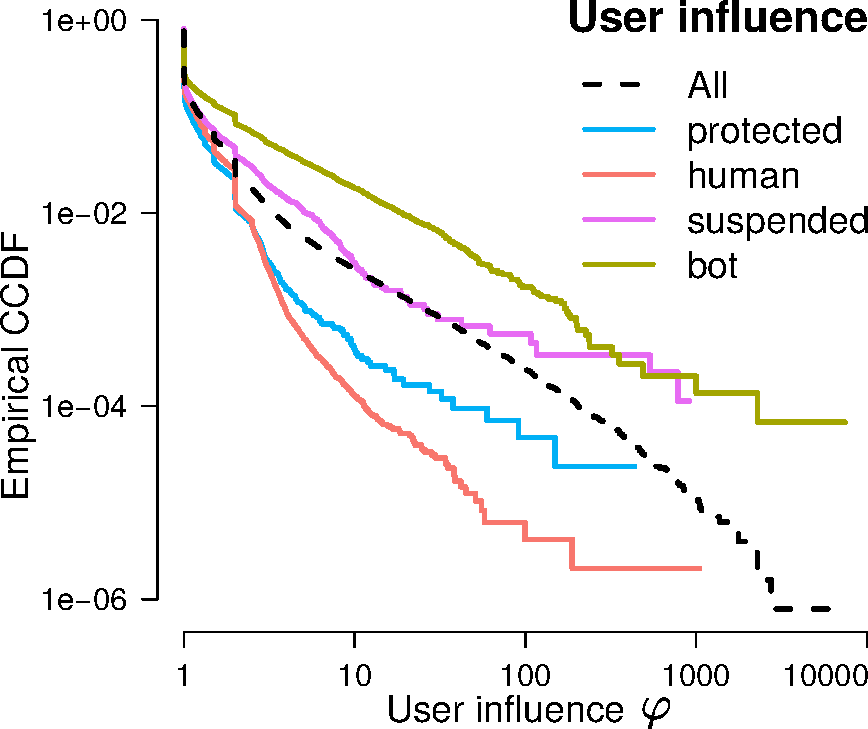
\includegraphics[height=\myheight\textheight]{2017-11-13-CCDF-influence-4-populations}
		\label{subfig:user-infl-CCDF}
	}
	\subfloat[] {
		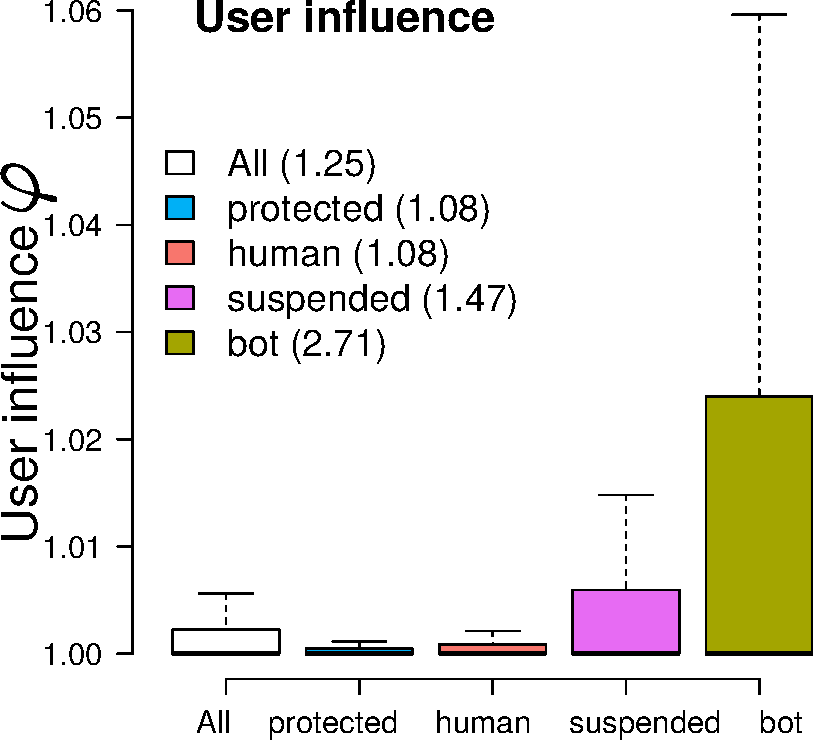
\includegraphics[height=\myheight\textheight]{2017-11-13-boxplot-influence-4-populations}
		\label{subfig:user-infl-boxplots}
	}
	\subfloat[] {
		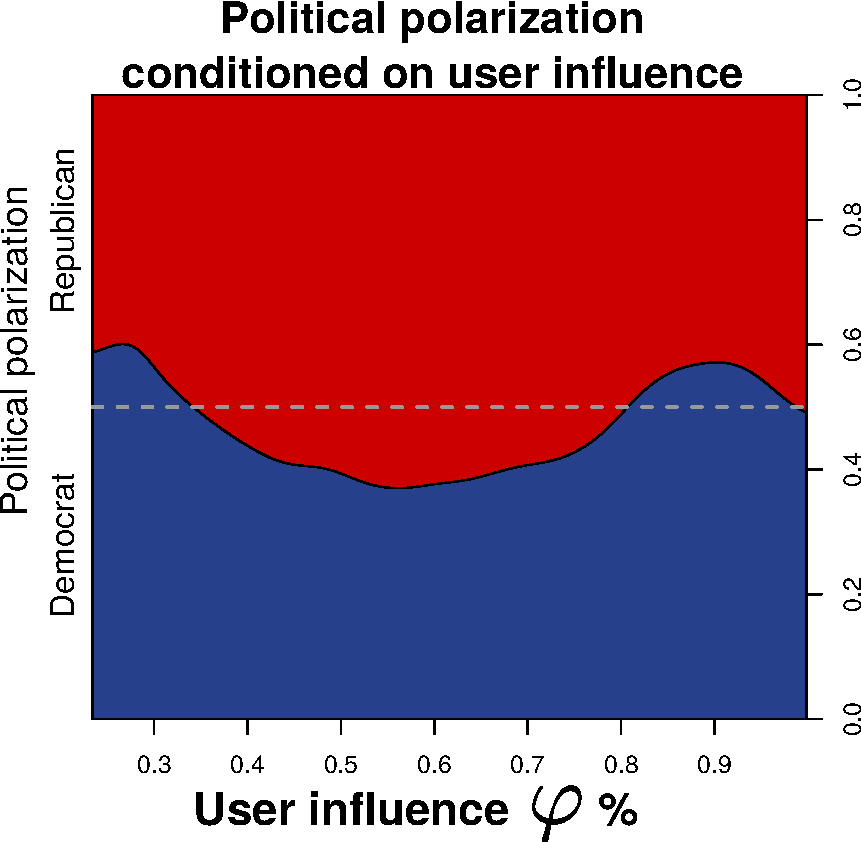
\includegraphics[height=\myheight\textheight]{influence_conditional_density}
		\label{subfig:polarization-conditioned-user-infl}
	}
	\subfloat[] {
		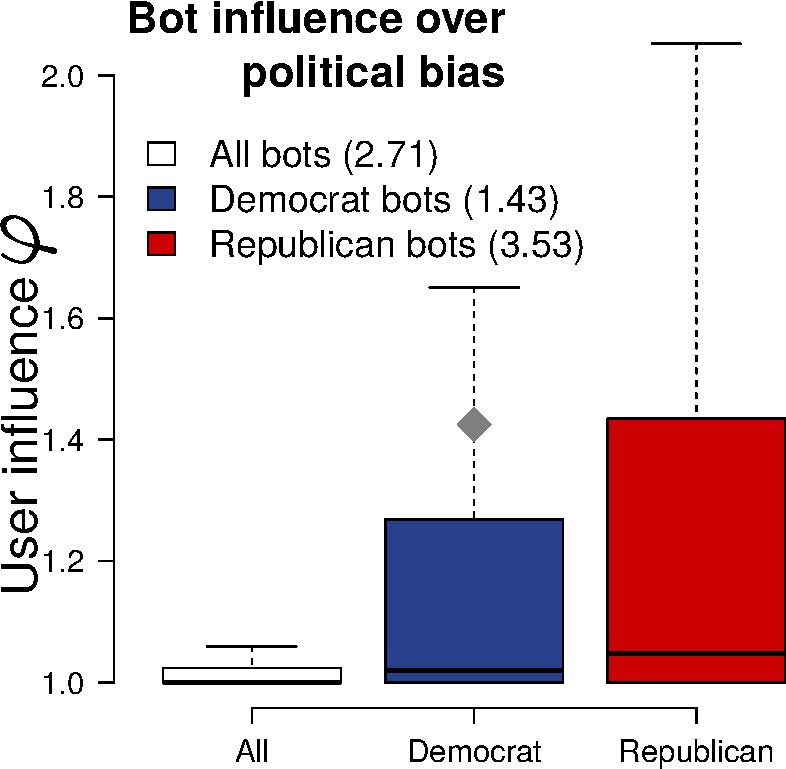
\includegraphics[height=\myheight\textheight]{BOTS_boxplot-influence-vs-political-bias}
		\label{subfig:bot-influence}
	}
	\caption{ 
		Profiling influence, and linking to botness and political behavior.
		\textbf{(a)(b)} User influence $\varphi(u)$ for the reference populations, shown as log-log CCDF plot (a) and boxplots (b).
%		The influence in each of the four reference populations is long-tail distributed.
%		\textbf{(b)} Boxplot of user influence for the four bot populations -- 
		\textbf{(c)} Probability distribution of polarization, conditional on $\varphi(u) \%$.
		\textbf{(d)} Boxplots of user influence for the pro-Democrat and pro-Republican \Bot users.
		% (dashed line), and for the democrat and republican polarized populations (blue and red lines respectively).
		%\TODO{MAR}{Message in text: republican bots are more engaged than democrat bots.}
		Numbers in parenthesis show mean values.
	}
%	\label{fig:holdout-ll}
%	\captionmoveup
\end{figure*}

%!TEX root = main.tex

\begin{figure}[tb]
	\centering
	
	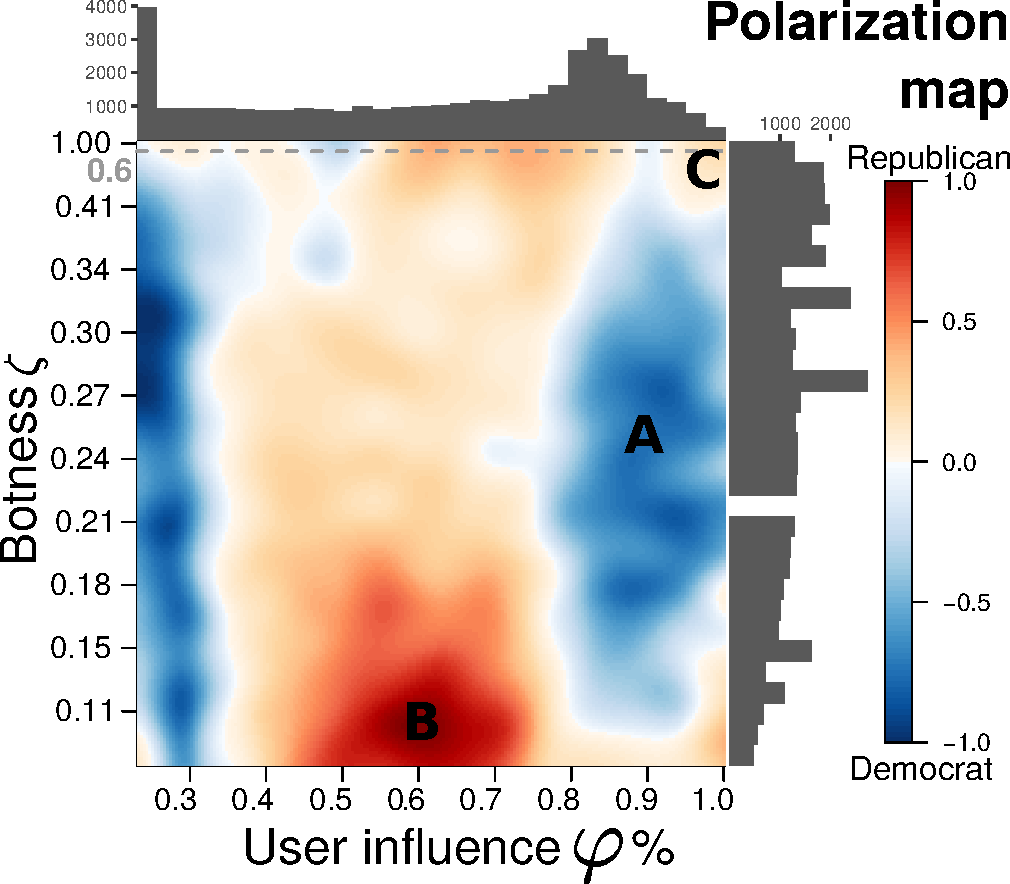
\includegraphics[width=0.47\textwidth]{influence-botscore-polarization-2d-map}

	\caption{ 
		Political polarization by user influence $\varphi(u) \%$ (x-axis) and bot score $\zeta$ (y-axis).
%		The x-axis shows the percentile of user influence, from 0 being the least influential to 1 being the most influential.
%		The y-axis shows the bot score. 
		% (see the distribution of bot score density in Fig.~\ref{subfig:botscore-density}).
		The gray dashed horizontal line shows the threshold of 0.6 above which a user is considered a bot.
		The color in the map shows political polarization: areas colored in bright blue (red) are areas where the Democrats (Republicans) have considerably higher density than Republicans (Democrats).
		%: it is the ratio of the density of Democrat users to the density of Republican users.
%		Areas where the density of Republicans is considerably higher than the density of Democrats are colored bright red (and similarly for bright blue).
		Areas where the two populations have similar densities are colored white.
		Three areas of interest are shown by the letter \textbf{A}, \textbf{B} and \textbf{C}.
	}
	\label{fig:polarization-map}
%	\captionmoveup
\end{figure}

\subsection{User influence and polarization map}
\label{subsec:user-influence-results}

\textbf{User influence across four populations.}
First, we study the distribution of user influence across the four reference populations constructed in Sec.~\ref{subsec:bot-detection}.
We plot the CCDF in Fig.~\ref{subfig:user-infl-CCDF} and we summarize user influence as boxplots in Fig.~\ref{subfig:user-infl-boxplots} for each population.
User influence $\varphi$ is long-tail distributed (shown in Fig.~\ref{subfig:user-infl-CCDF}) and it is higher for \Bot and \Suspended populations, than for \Human and \Protected (shown in Fig~\ref{subfig:user-infl-boxplots}).
There is a large discrepancy between the influence of \Human and \Bot (p-val $= 0.0025$), with \emph{the average bot having 2.5 times more influence than the average human.}
%\TODO{MAR}{Message in text: bots have higher user influence.}
We further break down users in the \Bot population based on their political polarization.
Fig.~\ref{subfig:bot-influence} aggregates as boxplots the influence of pro-Democrat and pro-Republican bots (note: not all bots are politically polarized).
Notably, on a per-bot basis, pro-Republican bots are more influential than their pro-Democrat counterparts (p-val $= 0.0096$) -- \emph{the average pro-Republican bot is twice as influential as the average pro-Democrat bot}.
%\TODO{MAR}{Message in text: republican bots are more influential than democratic bots.}

\textbf{Political polarization and user influence.}
Next, we analyze the relation between influence and polarization.
Fig.~\ref{subfig:polarization-conditioned-user-infl} plots the probability distribution of political polarization, conditioned on user influence $\varphi \%$.
While for mid-range influential users ($\varphi \% \in [0.4, 0.8]$) the likelihood of being Republican is higher than being Democrat, we observe the inverse situation on the higher end of the influence scale.
\emph{Very highly influential users ($\varphi \% > 0.8]$) are more likely to be pro-Democrat}, and this is consistent with the fact that many public figures were supportive of the Democrat candidate during the presidential campaign.
%\TODO{MAR}{Message in text: highly influential users are likely to be democrats -- mobilization of civil society.}

\textbf{The polarization map.}
Finally, we create a visualization that allows us to jointly account for botness and user influence when studying political partisanship.
We project each politically polarized user in \debate onto the two-dimensional space of user influence $\varphi \%$ (x-axis) and botness $\zeta$ (y-axis).
The y-axis is re-scaled so that an equal length interval around any botness value contains the same amount of users,
This allows to zoom in into denser areas like $\zeta \in [0.2, 0.4]$, and to deal with data sparsity around high botness scores.
We compute the 2D density estimates for the pro-Democrat and pro-Republican users (shown in the online supplement~\cite[annex~E]{supplemental}).
%\ref{si-sec:polarization-map}
%While these allow to identify dense and sparse regions, for one polarization or the other, in order to show both 
For each point in the space $(\varphi \%, \zeta)$ we compute a score as the log of the ratio between the density of the Republican users and that of the pro-Democrats, which is then renormalized so that values range from -1 (mostly Democrat) to +1 (mostly Republican).
The resulting map -- dubbed the \emph{polarization map} -- is shown in Fig.~\ref{fig:polarization-map} and it provides a number of insights.
Three areas of interest (\textbf{A}, \textbf{B} and \textbf{C}) are shown on Fig.~\ref{fig:polarization-map}.
Area \textbf{A} is a pro-Democrat area corresponding to highly influential users (already shown in Fig.~\ref{subfig:polarization-conditioned-user-infl}) that spans across most of the range of botness values.
Area \textbf{B} is the largest predominantly pro-Republican area and it corresponds to mid-range influence (also shown in Fig.~\ref{subfig:polarization-conditioned-user-infl}) and concentrates around small botness values -- this indicates the presence of a large pro-Republican population of mainly human users with regular user influence.
Lastly, we observe that the top-right area \textbf{C} (high botness and high influence) is predominantly red: 
%are more likely to be \rvt{pro-Republican}.
In other words \emph{highly influential bots are mostly pro-Republican.}